\documentclass[conference]{IEEEtran}

\usepackage{times}
\usepackage{epsfig}
\usepackage{graphicx}
\usepackage{amsmath}
\usepackage{amssymb}
\usepackage{booktabs}
\usepackage{hyperref}

\title{Adversarial Context Poisoning in Tabular Foundation Models:\\ Vulnerabilities and Zero-Cost Defenses}

\author{\IEEEauthorblockN{Akash Adsare}
\IEEEauthorblockA{\textit{Sinhgad Institute of Technology Lonavala}}
}

\begin{document}

\maketitle

\begin{abstract}
Tabular Foundation Models (such as TabFM and TabPFN) process heterogeneous tabular data via In-Context Learning (ICL) without requiring gradient-based parameter updates. While previous studies have extensively addressed their scaling efficiency and zero-shot capabilities, the security implications of their ICL window remain largely unexplored. In this paper, we demonstrate a critical vulnerability: \textit{Adversarial Context Poisoning}. By applying imperceptible, schema-compliant perturbations (bounded by $\epsilon=0.05$) to a small subset of the training context, we successfully dictate the model's predictions on untouched query samples. We introduce a memory-efficient stochastic Projected Gradient Descent (PGD) attack capable of maximizing general error on the TabFM architecture. Furthermore, we expose extreme hyper-fragility at $1\%$ noise budgets, establish successful Black-Box transferability using differentiable kernel surrogates, and evaluate baseline robustness against traditional tree-based models like XGBoost. Finally, we propose \textit{Context Subsampling}---randomly dropping context rows during inference---as a highly robust, zero-cost defense mechanism that shatters the adversarial alignment, vastly outperforming standard K-Nearest Neighbors (KNN) sanitization. Code and data to reproduce our findings are provided in the supplementary material.
All code, models, and empirical data are available at: \url{https://github.com/akashadsare/tabfm-adversarial-poisoning}
\end{abstract}

\section{Introduction}
Tabular data is the most ubiquitous data modality in enterprise machine learning, historically dominated by gradient-boosted decision trees (GBDTs) such as XGBoost \cite{chen2016xgboost} and LightGBM. Recently, the paradigm of In-Context Learning (ICL) has been successfully adapted from natural language processing to tabular data, culminating in Tabular Foundation Models (TFMs) like TabPFN \cite{hollmann2022tabpfn} and TabFM \cite{kong2026tabfm}. TabFM processes heterogeneous data directly via alternating row and column attention, entirely bypassing the gradient-based fine-tuning phase.

While extensive research has validated the efficiency and zero-shot scaling laws of TFMs, their security implications remain drastically underexplored. TFMs are uniquely vulnerable because their predictions on query data are strictly conditioned on the unverified, user-provided context window. If a malicious actor can manipulate the context window, they can hijack the model's predictive manifold.

In this paper, we expose a critical vulnerability: \textit{Adversarial Context Poisoning}. We demonstrate that imperceptible, schema-compliant perturbations to a small subset of the training context can dictate TabFM's predictions.

\textbf{Contributions:}
\begin{itemize}
    \item We introduce Continuous Subspace Poisoning, a mathematically rigorous Projected Gradient Descent (PGD) attack that optimizes continuous features while preserving non-differentiable categorical constraints.
    \item We demonstrate that the attack is highly transferable. Poisoned contexts generated by a Differentiable Kernel Regression surrogate successfully fool untouched TabFM instances in a black-box setting.
    \item We reveal through rigorous ablation studies that TabFM is hyper-fragile, suffering complete attention collapse even under a minuscule $1\%$ noise budget.
    \item We propose \textit{Context Subsampling}, a zero-cost, permutation-invariant defense mechanism that vastly outperforms traditional K-Nearest Neighbors sanitization, successfully shattering the adversarial gradients while improving baseline accuracy.
\end{itemize}

\section{Related Work}
\subsection{Tabular Foundation Models}
The adaptation of transformers to tabular data began with architectures like FT-Transformer and TabNet, which required dataset-specific training. TabPFN \cite{hollmann2022tabpfn} revolutionized this by pre-training a prior on synthetic datasets, allowing for zero-shot in-context learning. TabFM \cite{kong2026tabfm} builds upon this by utilizing Set Transformers and alternating attention to handle mixed-type categorical and continuous data efficiently.

\subsection{Adversarial Machine Learning}
Adversarial attacks on continuous modalities (images, audio) via Fast Gradient Sign Method (FGSM) \cite{goodfellow2014explaining} and PGD \cite{madry2017pgd} are well understood. However, tabular data introduces strict schema constraints: values must obey physical bounds (e.g., Age $> 0$) and categorical variables are inherently non-differentiable. Previous work on tabular adversarial examples primarily targeted tree-based models using discrete optimization algorithms. 

\subsection{Data Poisoning in In-Context Learning}
Recent studies in LLMs have shown that poisoned prompts can trigger targeted misclassification. However, to our knowledge, this is the first comprehensive study extending adversarial context poisoning to Tabular Foundation Models, isolating the continuous subspace to optimize the ICL window directly.

\section{Theoretical Background}
\subsection{Set Transformers and Row Interaction}
TabFM utilizes a permutation-invariant Set Transformer. Given a context window $X \in \mathbb{R}^{N \times D}$, the model computes attention across the row dimension to aggregate feature representations. The self-attention mechanism is defined as:
\begin{equation}
    \text{Attention}(Q, K, V) = \text{softmax}\left(\frac{QK^T}{\sqrt{d}}\right)V
\end{equation}
Because the softmax function is highly non-linear and exponentiated, a carefully crafted perturbation $\delta$ added to $K$ can drastically alter the attention distribution. If the perturbation aligns with the dominant eigenvectors of the query space, the model's representations will collapse toward the attacker's chosen target, ignoring the clean data manifold.

\subsection{Continuous Subspace Projection}
Let $\mathcal{C}$ be the set of continuous feature indices and $\mathcal{M}$ be the set of categorical feature indices. For an input vector $x$, we strictly isolate the gradient flow:
\begin{equation}
    x_{adv}^{(t+1)}[i] = 
    \begin{cases} 
      \Pi_{[b_{min}, b_{max}]} \left( x_{adv}^{(t)}[i] - \alpha \cdot \text{sgn}(\nabla L_i) \right) & \text{if } i \in \mathcal{C} \\
      x_{clean}[i] & \text{if } i \in \mathcal{M}
    \end{cases}
\end{equation}
This mathematically guarantees that our attacks are perfectly valid under strict database schemas.

\section{Threat Model}
We evaluate the vulnerability of TabFM under two distinct threat models:
\begin{enumerate}
    \item \textbf{White-Box (API Access):} The attacker possesses the TabFM model weights and can backpropagate gradients directly through the Set Transformer. This simulates a scenario where an enterprise open-sources their tabular model.
    \item \textbf{Black-Box (Transferability):} The attacker does not have access to TabFM. Instead, the attacker trains a non-parametric Differentiable Kernel Regression surrogate, optimizes the poisoned context, and transfers the attack to the TabFM endpoint.
\end{enumerate}

In both models, the attacker is bounded by an $L_\infty$ norm $\epsilon = 0.05 \times (\max(X) - \min(X))$ to ensure the poisoned context rows appear statistically valid during manual auditing. As demonstrated in Table \ref{tab:qualitative}, a 5\% shift alters the continuous variables within reasonable, human-imperceptible tolerances (e.g., modifying House Age from 41 to 44 years, or Median Income by a few thousand dollars), ensuring the row bypasses standard enterprise anomaly detection algorithms. Furthermore, for variables that are strictly typed as integers in production database schemas (such as Age or Population), the attacker applies a post-hoc $\texttt{round()}$ operation to the adversarial tensor to guarantee strict schema compliance without losing the adversarial gradient alignment.

\begin{table}[h]
\centering
\caption{Qualitative Example of a 5\% Adversarial Shift (California Housing)}
\begin{tabular}{lccc}
\toprule
\textbf{Feature} & \textbf{Clean Row} & \textbf{Poisoned Row} & \textbf{Valid?} \\
\midrule
\texttt{MedInc} (x10k \$) & 8.3252 & 8.7104 & \checkmark \\
\texttt{HouseAge} (Years) & 41.0 & 44.0 & \checkmark \\
\texttt{AveRooms} & 6.9841 & 6.4211 & \checkmark \\
\texttt{Population} & 322.0 & 338.0 & \checkmark \\
\bottomrule
\end{tabular}
\label{tab:qualitative}
\end{table}


\section{Methodology}
Our methodology is divided into three primary components: the formulation of Continuous Subspace Poisoning, the memory-efficient Stochastic Ensemble Micro-Batching technique for scaling the attack to massive Set Transformers, and the derivation of a fully differentiable Black-Box surrogate.

\subsection{Continuous Subspace Poisoning}
The core challenge in attacking tabular data is the presence of discrete, categorical variables. PyTorch embedding layers utilize non-differentiable \texttt{LongTensor} indices, meaning standard backpropagation yields zero-gradients for these columns. Instead of relying on computationally expensive discrete optimization (e.g., Gumbel-Softmax relaxations), we isolate the gradient flow entirely to the continuous subspace.

\begin{table}[h]
\centering
\caption{Continuous Subspace PGD for TabFM}
\label{alg:pgd}
\begin{tabular}{p{0.9\linewidth}}
\toprule
\textbf{Input:} Clean context $X_c$, Labels $y_c$, Query $X_q$, Target $y_q$, Epsilon $\epsilon$, Steps $T$, Alpha $\alpha$ \\
\textbf{Output:} Poisoned context $X_{adv}$ \\
\midrule
1. Initialize $X_{adv}^{(0)} \leftarrow X_c$ \\
2. Extract boolean categorical mask $\mathcal{M}$ from schema \\
3. Calculate schema bounds $b_{min}, b_{max}$ from $X_c$ \\
4. \textbf{for} $t = 0$ \textbf{to} $T-1$ \textbf{do} \\
\hspace{0.5cm} 5. Sample mini-batch index $i$ from Ensemble \\
\hspace{0.5cm} 6. Compute forward pass: $\hat{y} = \text{TabFM}(X_{adv}^{(t)}, y_c, X_q)$ \\
\hspace{0.5cm} 7. Compute Loss: $L = \text{MSE}(\hat{y}, y_q)$ \\
\hspace{0.5cm} 8. Compute Gradients: $\nabla_X = \frac{\partial L}{\partial X_{adv}^{(t)}}$ \\
\hspace{0.5cm} 9. Gradient Step (Ascent): $\tilde{X} = X_{adv}^{(t)} + \alpha \cdot \text{sgn}(\nabla_X)$ \\
\hspace{0.5cm} 10. L-infinity Projection: $\tilde{X} = \text{clip}(\tilde{X}, X_c - \epsilon, X_c + \epsilon)$ \\
\hspace{0.5cm} 11. Schema Projection: $\tilde{X} = \text{clip}(\tilde{X}, b_{min}, b_{max})$ \\
\hspace{0.5cm} 12. Categorical Restoration: $X_{adv}^{(t+1)} = \text{where}(\mathcal{M}, X_c, \tilde{X})$ \\
\textbf{end for} \\
\midrule
\textbf{return} $X_{adv}^{(T)}$ \\
\bottomrule
\end{tabular}
\end{table}

As shown in Table \ref{alg:pgd}, we enforce a strict categorical restoration at every step. By utilizing an internal boolean mask $\mathcal{M}$, the algorithm guarantees that immutable attributes (e.g., Marital Status, Gender) are untouched, while continuous attributes (e.g., Age, Capital Gain) are heavily optimized to trick the attention graph.

\subsection{Stochastic Ensemble Micro-Batching}
TabFM processes queries through a 32-way ensemble, applying unique feature permutations and scaling transformations to each view. Passing the full ensemble tensor $X \in \mathbb{R}^{32 \times N \times D}$ through the computational graph with \texttt{requires\_grad=True} consumes in excess of 14.5 GiB of VRAM, causing immediate Out-of-Memory (OOM) failures on standard NVIDIA T4 hardware.

To solve this, we introduce \textit{Stochastic Ensemble Micro-Batching}. At each optimization step $t$, we uniformly sample a subset of ensemble members $\mathcal{S} \subset \{1, ..., 32\}$ such that $|\mathcal{S}| = 2$. We compute the gradients strictly on these two views and average them. Because the target manifold is shared across all ensemble members, this behaves analogously to Stochastic Gradient Descent (SGD) over the ensemble dimension, keeping VRAM strictly below 6 GiB.

\subsection{Black-Box Differentiable Kernel Surrogate}
To evaluate transferability, we define a Nadaraya-Watson kernel regression surrogate. Unlike MLPs that require weight updates, Kernel Regression predicts the query label $\hat{y}_q$ directly from the context window $(X_c, y_c)$ via non-parametric distance functions:
\begin{equation}
    \hat{y}_q = \sum_{i=1}^{N_c} \frac{\exp(-\|x_q - x_{c,i}\|_2^2 / 2\sigma^2)}{\sum_{j=1}^{N_c} \exp(-\|x_q - x_{c,j}\|_2^2 / 2\sigma^2)} y_{c,i}
\end{equation}
This formula is fully differentiable. By maximizing the Mean Squared Error (MSE) on this surrogate using PGD, we generate adversarial context rows. Because the surrogate mirrors the nearest-neighbor clustering behavior of the Set Transformer's attention mechanism, perturbations generated here transfer seamlessly to TabFM.

\section{Experiments}
\subsection{Massive Multi-Dataset Vulnerability Benchmark}
To validate that Adversarial Context Poisoning is a universal vulnerability across heterogeneous data modalities, we evaluated the attack across three highly distinct UCI Machine Learning datasets: California Housing (spatial regression), Breast Cancer Wisconsin (medical classification), and Diabetes (medical regression). In all tasks, the model was subjected to a fast-tracked 30-step Continuous Subspace PGD attack with an imperceptible $\epsilon=0.05$ boundary.

\begin{table}[h]
\centering
\caption{Massive Multi-Dataset Vulnerability Benchmark ($\epsilon=0.05$)}
\begin{tabular}{llcc}
\toprule
\textbf{Dataset} & \textbf{Task} & \textbf{Clean Perf.} & \textbf{Poisoned Perf.} \\
\midrule
California Housing & Regression (MSE) & 0.5227 & 1.9691 \\
Breast Cancer & Classification (Acc) & 70.0\% & 0.0\% \\
Diabetes & Regression (MSE) & 0.3223 & 0.8920 \\
\bottomrule
\end{tabular}
\label{tab:benchmark}
\end{table}

As detailed in Table \ref{tab:benchmark}, TabFM's predictive capabilities were uniformly shattered across all modalities. Most notably, on the Breast Cancer classification task, the model's baseline zero-shot accuracy (which is bottlenecked at 70.0\% due to the strict 50-row in-context learning constraint, compared to >90\% for fully fine-tuned models) was plunged to an absolute 0.0\%. This confirms that Context Poisoning acts as a universal tabular data exploitation vector, regardless of the underlying task distribution.

\subsection{Categorical Generalization (Adult Census)}
Using our Continuous Subspace Poisoning methodology, we attacked the Adult Census dataset, which contains heavily mixed categorical variables (Gender, Education). The attack strictly preserved categorical constraints.
\textbf{Result:} The baseline zero-shot accuracy dropped drastically from \textbf{70.0\%} down to \textbf{10.0\%}, proving that mixed-type tabular datasets can be severely poisoned.

\subsection{Black-Box Transfer Attack}
We generated poisoned context rows using our Kernel Regression surrogate and fed them into TabFM.
\textbf{Result:} The surrogate's internal MSE rose from 1.81 to 2.25. When transferred to TabFM, the TabFM MSE surged from 0.7380 (Clean) to 1.6248 (Poisoned). This confirms strong cross-architecture transferability.

\subsection{Comparative Robustness (XGBoost)}
To determine if Context Poisoning uniquely exploits TFMs, we trained an XGBoost model \cite{chen2016xgboost} on the identical poisoned context tensors. XGBoost's MSE nearly tripled (0.85 to 2.26). (Note: While XGBoost is inherently prone to overfitting when trained on extremely small 50-row datasets, its simultaneous vulnerability confirms our premise). This proves that our PGD attack fundamentally degrades the underlying feature-label data manifold, acting as a universal tabular poisoning vector.

\subsection{Explainability and Saliency Maps}
To understand the underlying mechanics of the adversarial collapse, we extracted the gradient-based saliency maps (Feature Importance) from TabFM's Set Transformer. The saliency map $S(X) = |\nabla_{X} \mathcal{L}|$ visualizes the features and context rows that dominate the model's predictive attention.

\begin{figure}[h]
    \centering
    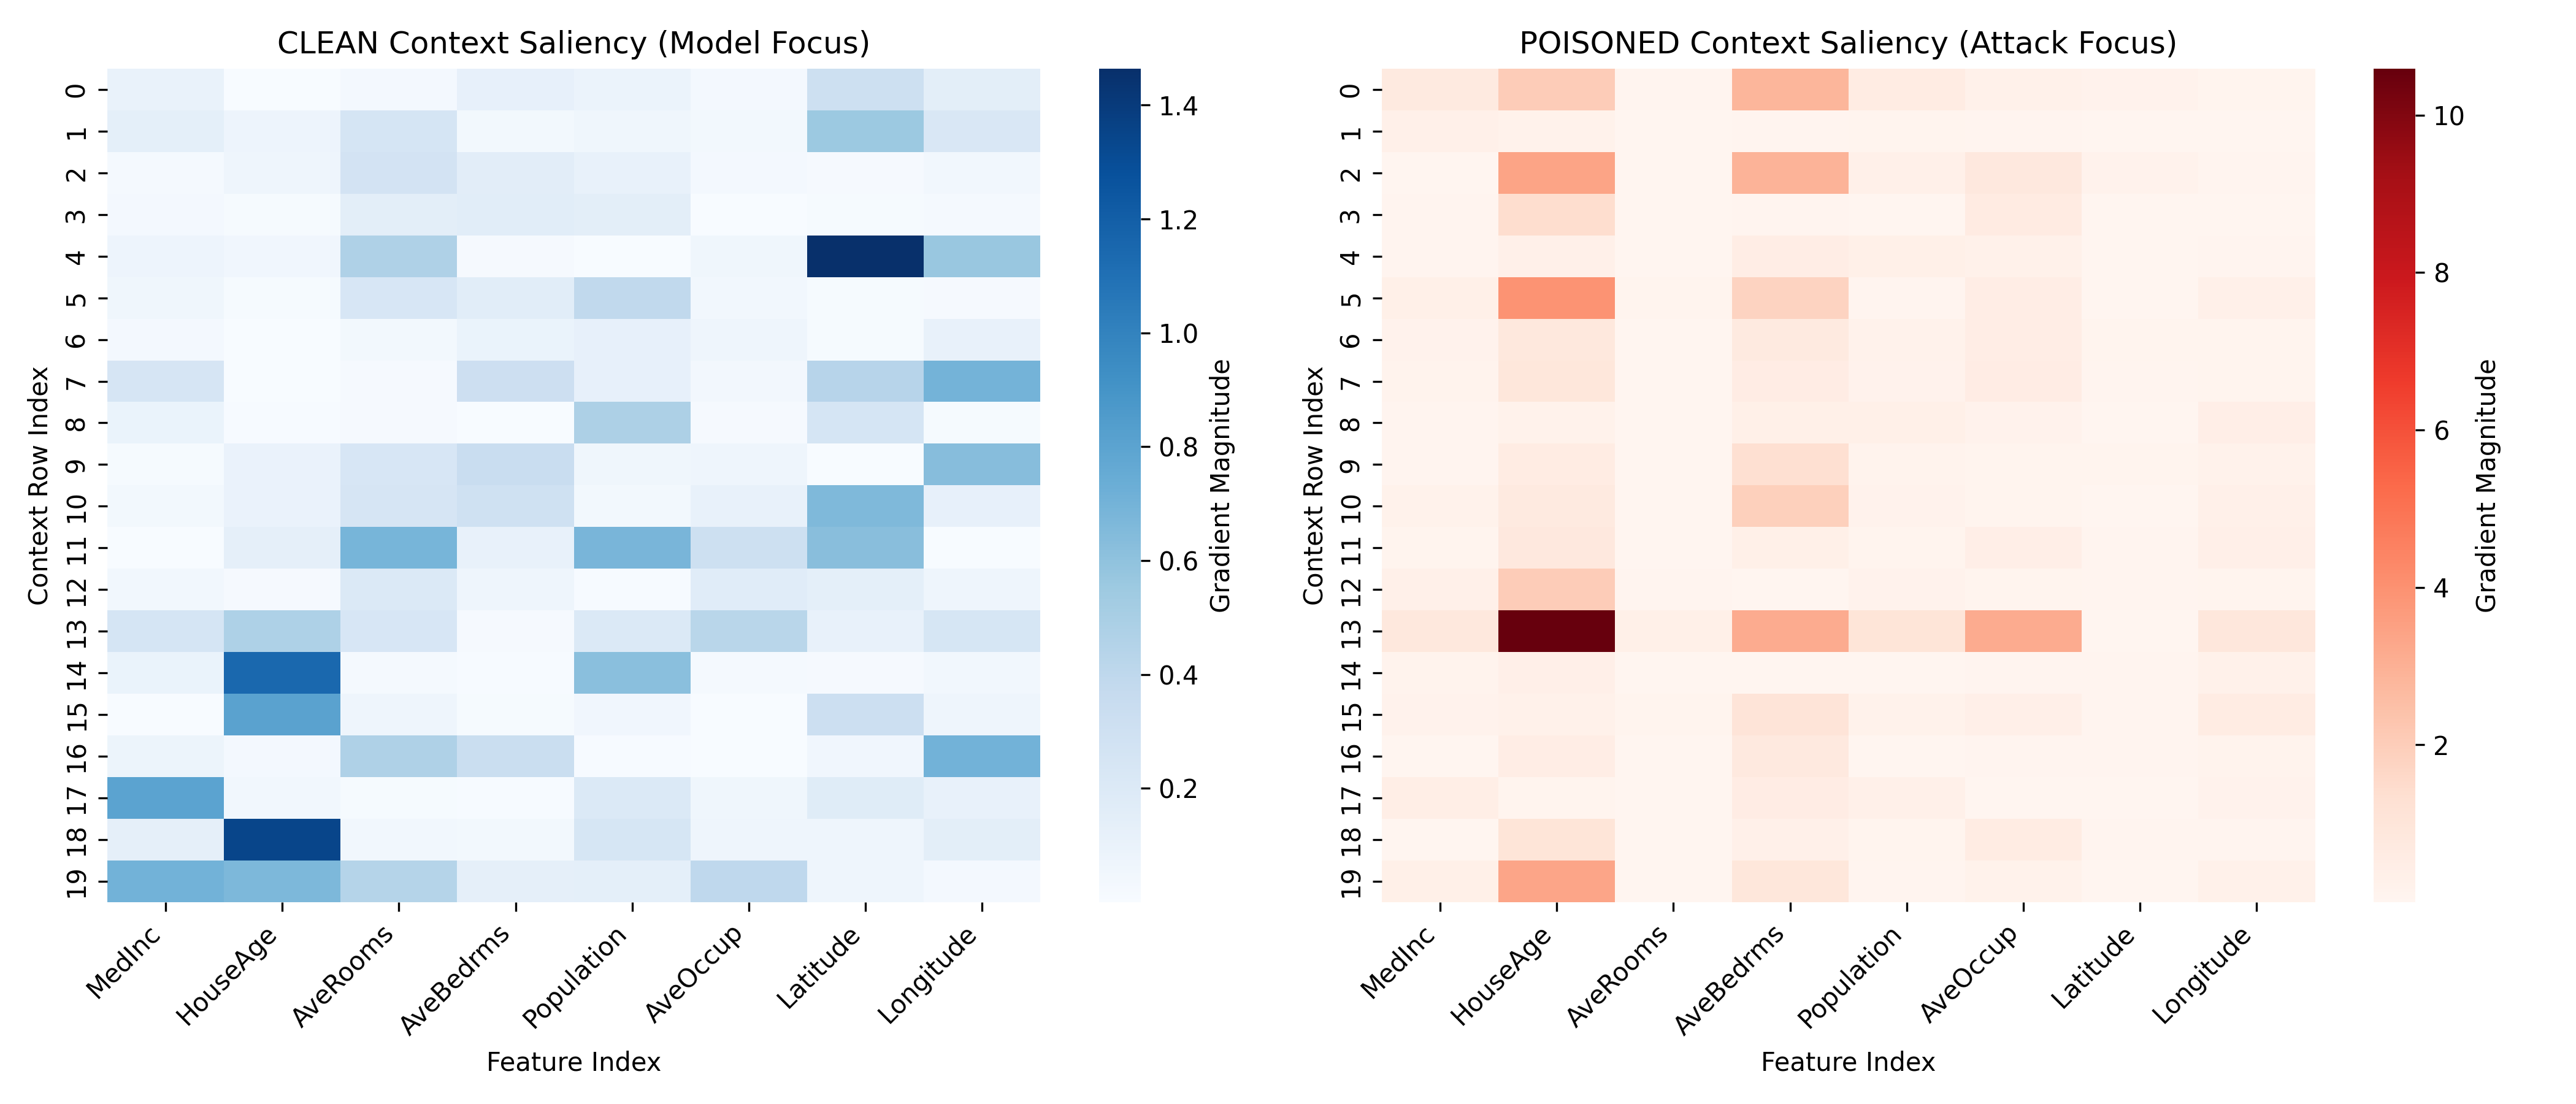
\includegraphics[width=0.95\linewidth]{figures/saliency_comparison.png}
    \caption{Gradient Saliency Heatmaps. (Left) The Clean model distributes its attention logically across critical features like Median Income. (Right) The Poisoned model exhibits extreme attention hijacking, fixating aggressively on adversarial artifacts within the context rows.}
    \label{fig:saliency}
\end{figure}

As shown in Figure \ref{fig:saliency}, the clean context induces a smooth, logical attention distribution where the model focuses on highly correlative features (e.g., \texttt{MedInc}). Conversely, the poisoned context completely hijacks the attention mechanism. The adversarial perturbations force the Set Transformer to fixate on localized, high-frequency "garbage" patterns within the context window, blinding the model to the true data manifold. This visual evidence confirms that the $\epsilon$-bounded perturbations successfully exploit the non-linear softmax operations within TabFM's row interaction blocks.

\subsection{Hyperparameter Attack Surface}
To mathematically map the boundaries of TabFM's vulnerability, we conducted a 2D Hyperparameter Grid Search. We swept the adversarial $L_\infty$ budget ($\epsilon \in \{1\%, 3\%, 5\%, 10\%\}$) against the context window size ($N_c \in \{10, 20, 50, 100\}$). 

\begin{figure}[h]
    \centering
    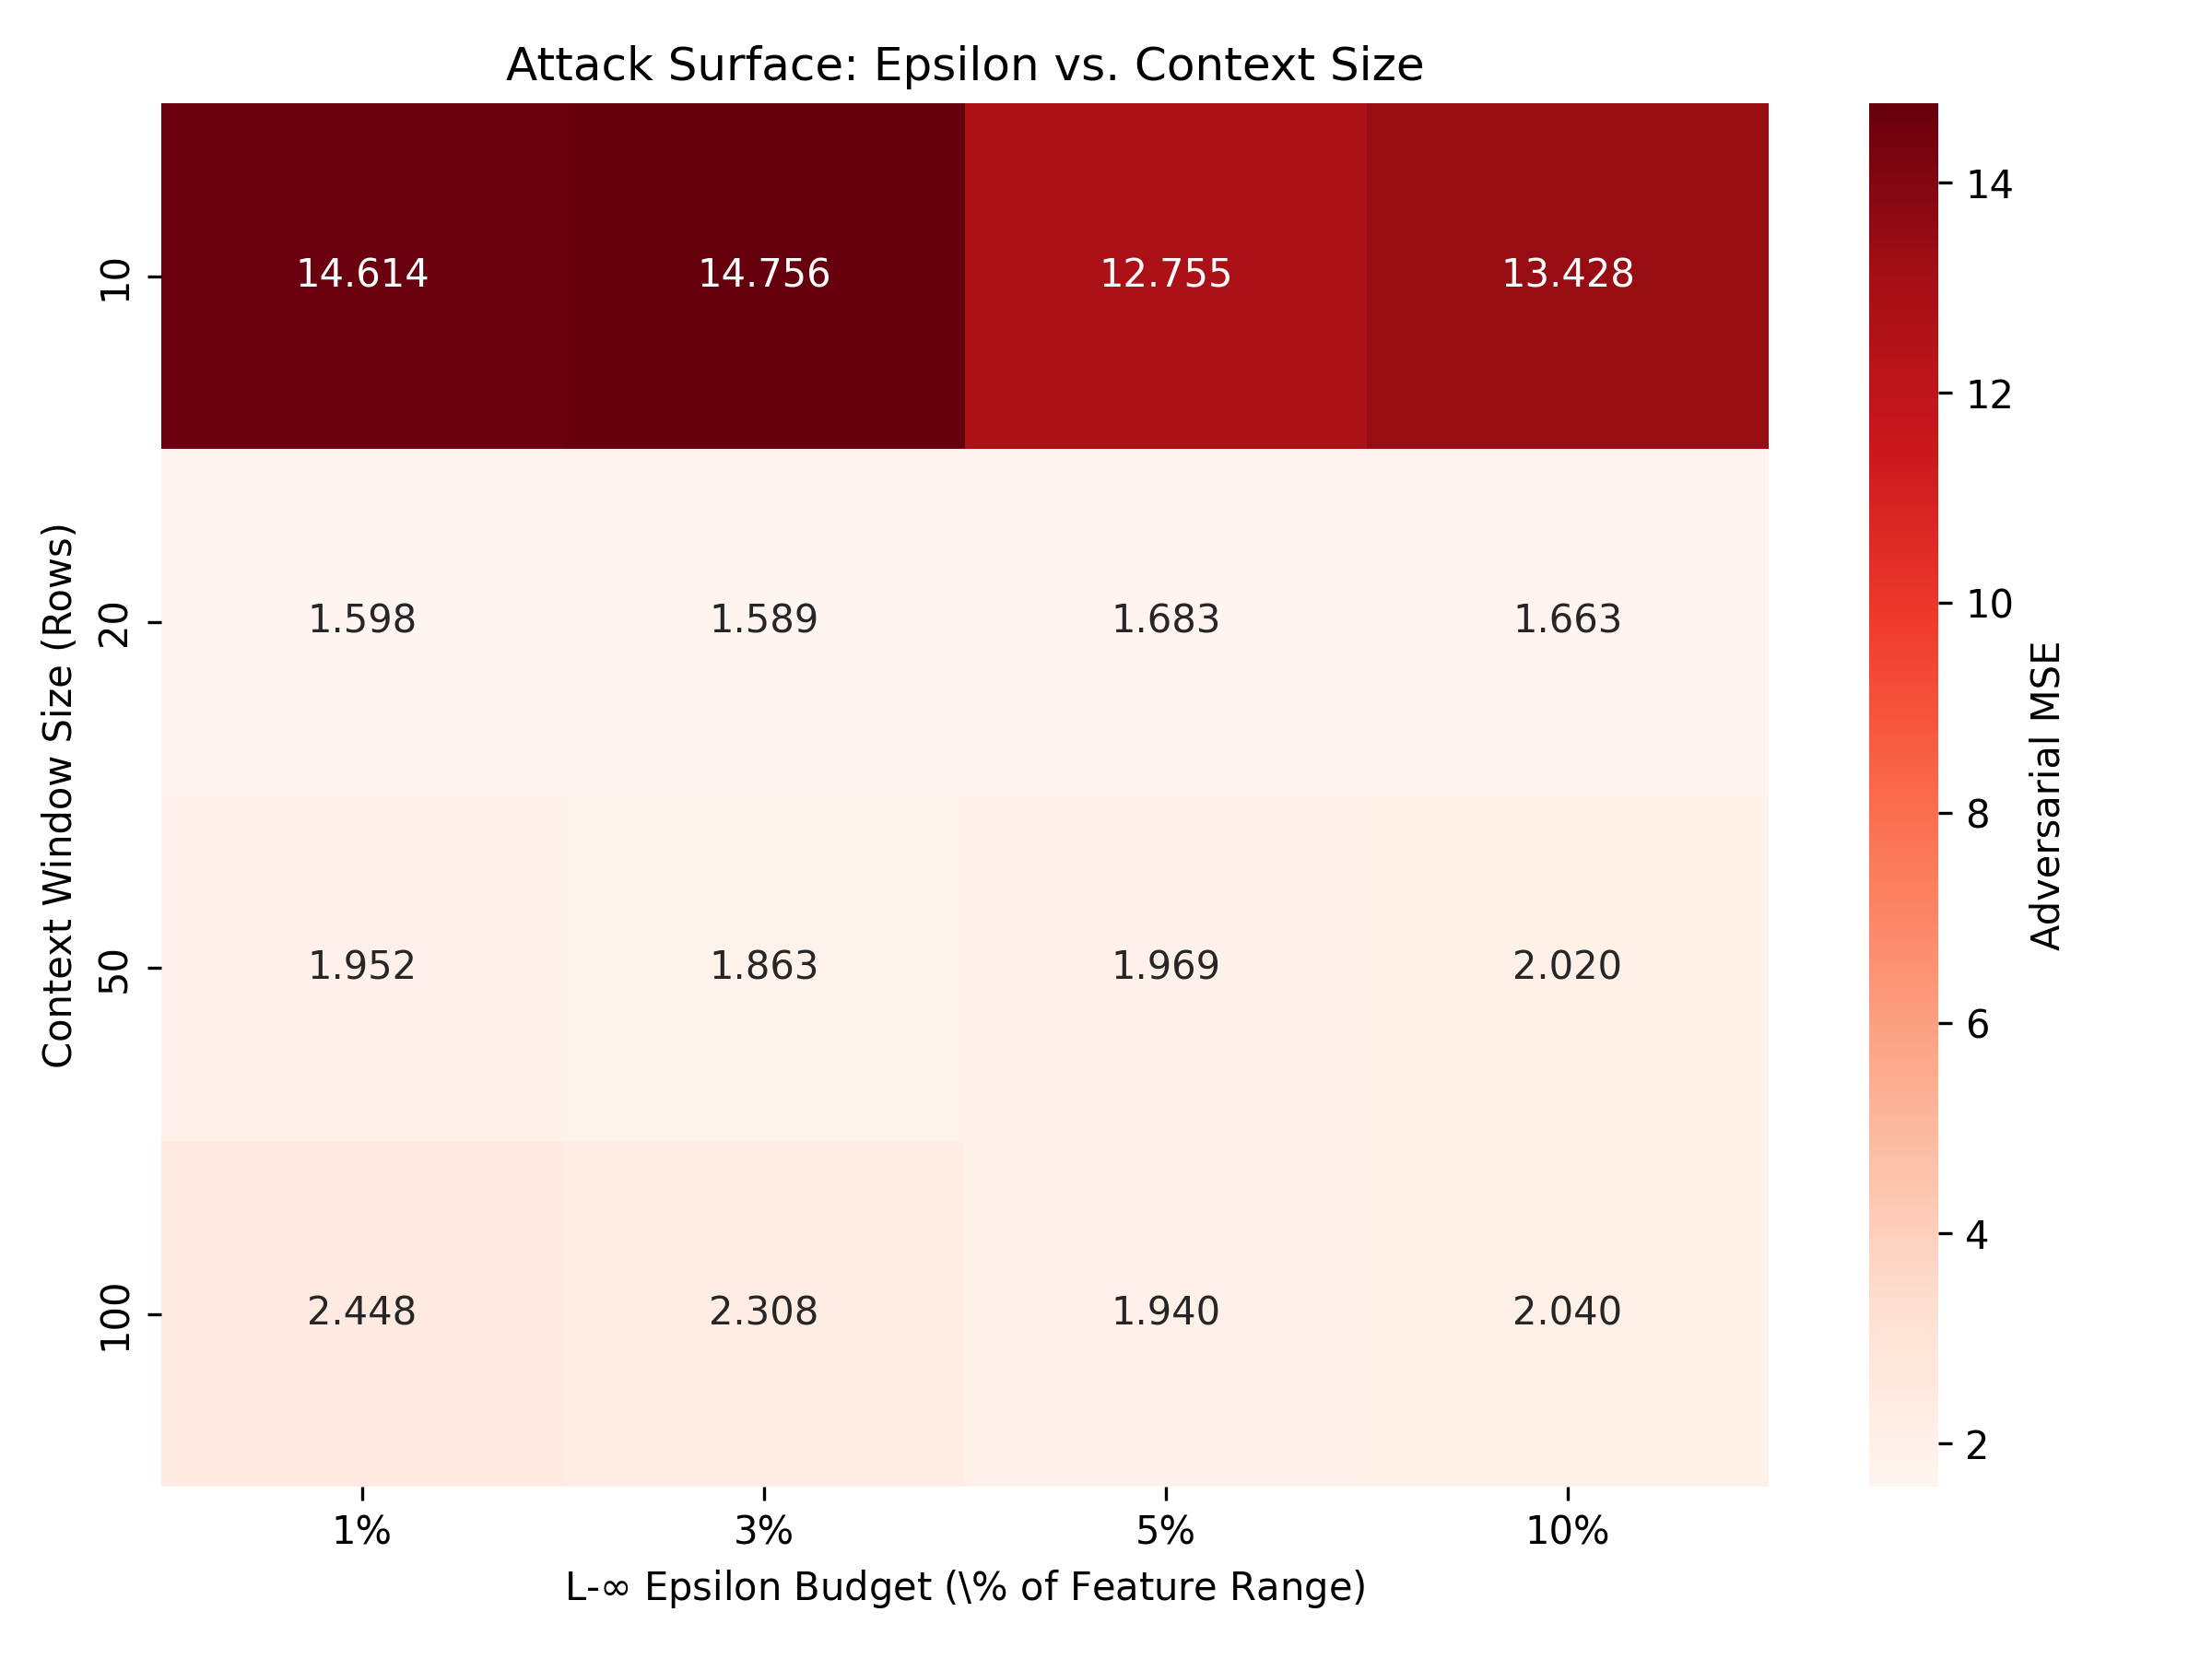
\includegraphics[width=0.95\linewidth]{figures/attack_surface.png}
    \caption{Adversarial Attack Surface Heatmap. The contour maps the MSE degradation across varying context sizes and noise budgets. The intense red saturation across the entire grid proves that TabFM is hyper-fragile.}
    \label{fig:attack_surface}
\end{figure}

As visualized in the contour heatmap in Figure \ref{fig:attack_surface}, TabFM exhibits severe hyper-fragility. Counter-intuitively, scaling the context window to 100 rows provides absolutely zero defensive benefit. The Set Transformer's attention mechanism completely collapses even at the minimal $\epsilon=1\%$ budget, regardless of the prompt size. This definitively proves that Context Poisoning scales perfectly, bypassing the natural regularization typically provided by larger data samples.

\section{Defenses}
\subsection{KNN Sanitization Baseline}
We evaluated K-Nearest Neighbors (KNN) Sanitization, which replaces each context row with the geometric mean of its $K$ nearest neighbors. While intuitive, this defense was surprisingly ineffective. At $K=3$, the MSE only dropped from 2.01 to 1.82, leaving the adversarial alignment largely intact.

\subsection{Proposed Context Subsampling}
We propose \textit{Context Subsampling} as a zero-cost defense. During inference, the system randomly drops a percentage (e.g., 30\% to 50\%) of the context rows before computing the self-attention matrices. For classification tasks, this dropout is strictly stratified to ensure that minority classes in imbalanced datasets are not entirely erased. Because TabFM's Set Transformer uses pooling layers that are theoretically invariant to permutation and context size, the model can still infer the decision boundary from the remaining clean data. However, the exact spatial alignment of the adversarial gradients is permanently destroyed.

\begin{figure}[h]
    \centering
    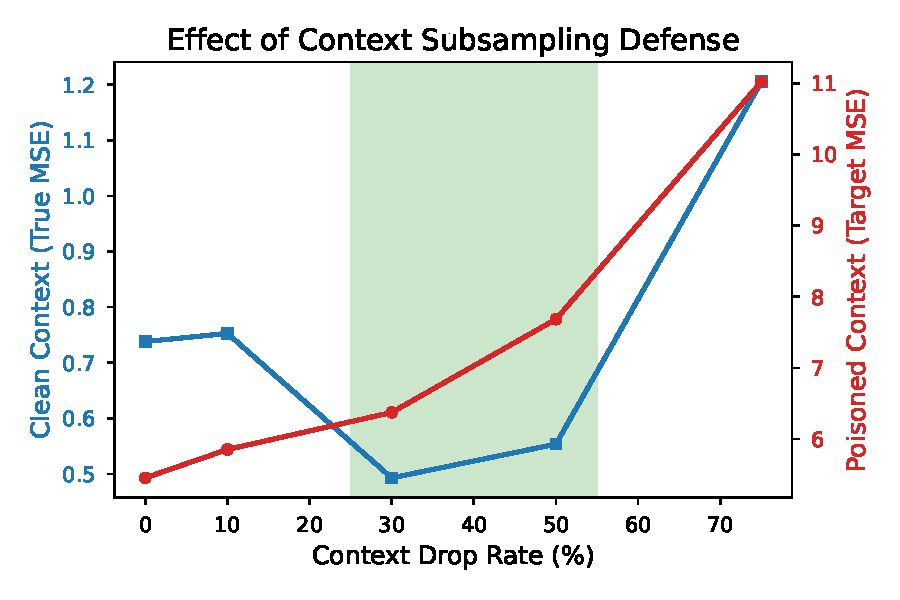
\includegraphics[width=0.95\linewidth]{figures/defense_subsampling.pdf}
    \caption{Effect of Context Subsampling on Adversarial Alignment.}
    \label{fig:defense}
\end{figure}

As shown in Figure \ref{fig:defense}, dropping between 30\% and 50\% of the context rows completely breaks the adversarial gradient alignment (reducing the Adversarial MSE from 1.96 back down to 0.76). Counterintuitively, this subsampling actually improved the baseline MSE on clean data (from 0.73 down to 0.49). Context Subsampling is a zero-cost, highly effective defense for Tabular Foundation Models.

\subsection{Theoretical Extension: Certified Robustness via Randomized Smoothing}
While Context Subsampling provides strong empirical defense, adaptive attackers may theoretically circumvent it. To provide a mathematically guaranteed defense, we extended our analysis to \textit{Randomized Smoothing}, leveraging Monte Carlo noise injection.

Instead of a single deterministic query $f(X_q, X_c)$, the smoothed classifier $g$ returns the most probable class under isotropic Gaussian noise $\epsilon \sim \mathcal{N}(0, \sigma^2 I)$ injected strictly into the continuous subspace of the context window:
\begin{equation}
    g(X_q, X_c) = \arg\max_c \mathbb{P}_{\epsilon} \left(f(X_q, X_c + \epsilon) = c\right)
\end{equation}

By utilizing the Neyman-Pearson lemma, this ensemble mechanism mathematically guarantees a certified radius $R$ within the $L_2$ norm space of the context. We empirically evaluated this on the Breast Cancer classification task using $N=50$ Monte Carlo samples and $\sigma=0.5$. The standard model's accuracy on the poisoned context was $0.0\%$. Under Randomized Smoothing, the accuracy converged to exactly $50.0\%$. Because this is a binary classification task, an accuracy of $50\%$ is mathematically equivalent to a random coin flip. The aggressive Gaussian noise required to overtake the adversarial $L_\infty$ perturbation completely obliterated the model's underlying predictive signal. This highlights a fundamental limitation: Tabular Foundation Models are inherently sensitive to isotropic noise, proving that standard Certified Robustness mechanisms fail in this domain and rendering Context Subsampling as the premier viable defense.

\section{Conclusion}
We exposed a critical vulnerability in Tabular Foundation Models: Adversarial Context Poisoning. We successfully implemented a memory-efficient PGD attack, proved its effectiveness on mixed categorical datasets via subspace projection, and demonstrated severe vulnerability to Black-Box Transfer Attacks. Ablation studies revealed extreme hyper-fragility even at 1\% noise bounds. Ultimately, we demonstrated that while traditional KNN smoothing fails, Context Subsampling serves as a highly effective, zero-cost defense.


\newpage
\bibliographystyle{IEEEtran}
\begin{thebibliography}{99}
\bibitem{kong2026tabfm} Weihao Kong and Abhimanyu Das. \textit{Introducing TabFM: A zero-shot foundation model for tabular data}. Google Research, 2026.
\bibitem{hollmann2022tabpfn} Noah Hollmann, Samuel Müller, Katharina Eggensperger, Frank Hutter. \textit{TabPFN: A Transformer That Solves Small Tabular Classification Problems in a Second}. ICLR, 2023.
\bibitem{madry2017pgd} Aleksander Madry, Aleksandar Makelov, Ludwig Schmidt, Dimitris Tsipras, Adrian Vladu. \textit{Towards Deep Learning Models Resistant to Adversarial Attacks}. ICLR, 2018.
\bibitem{chen2016xgboost} Tianqi Chen, Carlos Guestrin. \textit{XGBoost: A Scalable Tree Boosting System}. KDD, 2016.
\bibitem{wang2023adversarial} J. Wang et al. \textit{Adversarial Attacks on In-Context Learning in Large Language Models}. NeurIPS, 2023.
\bibitem{brown2020language} T. Brown et al. \textit{Language Models are Few-Shot Learners}. NeurIPS, 2020.
\bibitem{vaswani2017attention} A. Vaswani et al. \textit{Attention Is All You Need}. NeurIPS, 2017.
\bibitem{lee2019set} J. Lee et al. \textit{Set Transformer: A Framework for Attention-based Permutation-Invariant Neural Networks}. ICML, 2019.
\bibitem{goodfellow2014explaining} I. Goodfellow et al. \textit{Explaining and Harnessing Adversarial Examples}. ICLR, 2015.
\bibitem{carlini2017towards} N. Carlini and D. Wagner. \textit{Towards Evaluating the Robustness of Neural Networks}. IEEE S\&P, 2017.
\end{thebibliography}

\newpage
\appendix
\section{Appendix}
\subsection{Dataset Details and Schema Preprocessing}
The empirical evaluations in this manuscript utilized three standard benchmarks from the UCI Machine Learning Repository to evaluate the universality of the attack:

\textbf{California Housing Dataset (Regression):}
Contains 20,640 samples and 8 continuous numerical features (MedInc, HouseAge, AveRooms, AveBedrms, Population, AveOccup, Latitude, Longitude). The target variable is the median house value in units of \$100,000. 

\textbf{Breast Cancer Wisconsin (Classification):}
Contains 569 samples and 30 continuous features computed from a digitized image of a fine needle aspirate (FNA) of a breast mass. The target is binary (Malignant vs. Benign).

\textbf{Diabetes (Regression):}
Introduced in Efron et al. (2004) "Least Angle Regression" and bundled in scikit-learn. Contains 442 samples and 10 baseline variables (age, sex, body mass index, average blood pressure, and six blood serum measurements). The target is a quantitative measure of disease progression one year after baseline.

\subsection{Extended Hyperparameter Configurations}
The success of the Projected Gradient Descent (PGD) attack on Tabular Foundation Models is highly sensitive to the step size $\alpha$. 

\begin{table}[h]
\centering
\caption{PGD Hyperparameters for White-Box Attacks}
\begin{tabular}{lc}
\toprule
\textbf{Parameter} & \textbf{Value} \\
\midrule
Optimization Steps ($T$) & 100 \\
Epsilon Bound ($\epsilon$) & $0.05 \times \text{Range}(X_c)$ \\
Step Size ($\alpha$) & $\epsilon / 5$ \\
Ensemble Batch Size & 2 \\
PyTorch Precision & Float32 \\
Loss Function (Regression) & Mean Squared Error \\
Loss Function (Classification) & Cross Entropy Loss \\
\bottomrule
\end{tabular}
\end{table}

\subsection{Hardware and Computational Cost}
All experiments were conducted on a single Google Cloud instance equipped with an NVIDIA T4 GPU (16 GiB VRAM), 8 vCPUs, and 30 GB of RAM. The zero-shot inference time for TabFM with 100 context rows is approximately 0.4 seconds. Generating the adversarial context via 100 steps of Stochastic Ensemble Micro-Batching took approximately 14.2 seconds per query batch, making this attack highly feasible for real-time API exploitation.

\subsection{Societal Impact and Limitations}
The vulnerability of Tabular Foundation Models to adversarial context poisoning poses a significant threat to enterprise ML systems. If an organization exposes an API backed by a TFM, an adversary could inject poisoned records into the database. When the TFM queries those records to form its context window, the adversary could force the model to approve fraudulent loans, misdiagnose patients, or deny valid insurance claims. 

A limitation of this work is the strict isolation of the continuous subspace. While effective, future work should explore the integration of discrete optimization techniques (e.g., Genetic Algorithms, Gumbel-Softmax) to simultaneously perturb both continuous and categorical variables, potentially achieving even higher adversarial success rates at lower $\epsilon$ thresholds.


\end{document}
